\chapter{Iteración 4: Diseño final del Software} % (fold)
\label{cha:iteracion_4}

\section{Introducción} % (fold)
\label{it5:sec:introduccion}

En esta iteración, se intentó dar un cierre a un primer prototipo de software que cumpla con todos los requerimientos, o la mayor cantidad posible, teniendo en cuenta el riesgo intrínseco de cada uno.

Al final de la iteración 2, en la sección \ref{it2:sec:conclusiones_de_la_iteracion_2}, se especifica una lista con requerimientos cumplidos. Nuestro punto de partida para continuar el desarrollo del programa es esta lista. 

El objetivo principal de esta iteración es conformar un programa que cumpla con todos los requerimientos funcionales, inherentes al software de la plataforma.

% section introduccion (end)

\section{Requerimientos de la iteración} % (fold)
\label{it5:sec:requerimientos_de_la_iteracion}

Los requerimientos de esta iteración están planteados en base a los requerimientos principales, y los resultados de las pruebas y el desarrollo de la iteración 2. Además, se incluyen requerimientos nuevos, que surgieron por propuesta nuestra o de nuestro director, con motivo de mejorar las prestaciones de la plataforma.

\begin{itemize}
\item Se deberían poder configurar tiempos de intervalo entre cada medición para cada canal por separado (deriva de 1.5)
\item Se deberían poder guardar las configuraciones actuales en la memoria flash del microcontrolador, para poder restablecerlas en caso que el sistema se apague y se vuelva a prender. [4.1]
\item Se debería generar una marca de tiempo relativa al inicio de conversiones en cada medición realizada. [4.2]
\item Los datos que se envían a la placa de gestión para cada medición debería incluir, además de la medición, el numero de pin o pines (si es modo diferencial) de donde se esta midiendo. [4.3]
\item Los datos que se envían a la placa de gestión para cada medición debería incluir, además de la medición, el modo de conversión del canal por donde se esta midiendo. [4.4]
\item Los datos que se envían a la placa de gestión para cada medición debería incluir, además de la medición, la marca de tiempo relativa correspondiente de la medición hecha. [4.5] 
\end{itemize}


% section requerimientos_de_la_iteracion (end)

\section{Desarrollo} % (fold)
\label{it5:sec:desarrollo}

Focalizamos el desarrollo del programa en obtener un prototipo final, preparado para que se ejecute de manera continua en la placa de instrumentación construida. En una primera instancia, terminamos aquellas funcionalidades ligadas a los requerimientos principales, y luego nos dedicamos a comprobar el funcionamiento del mismo, mediante unit-testing y tests de sistema.

La Figura \ref{it5:fig:bloquesquintaiteracion} muestra el diagrama de bloques del programa terminado, al final esta iteración. Si se compara con la Figura \ref{it2:fig:bloquesprimeraiteracionsoftware}, el cambio en la estructura no es significativo. El mayor cambio esta en las funciones dentro de los bloques. Hay funciones nuevas, funciones que sufrieron cambios y funciones que se eliminaron.

\begin{figure}[h]
  \centering
  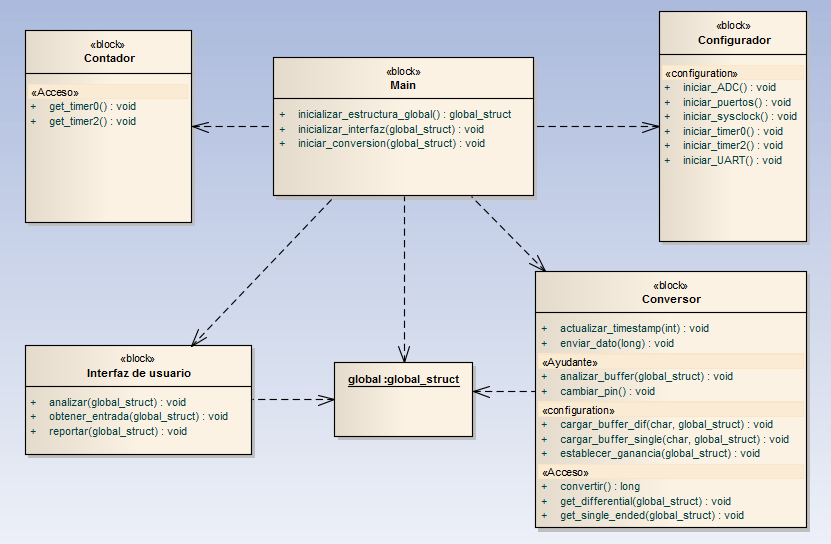
\includegraphics[width=1\textwidth, height = 10cm]{bloquesquintaiteracion}
  \caption{}\label{it5:fig:bloquesquintaiteracion}
\end{figure}

\subsection{Conversor} % (fold)
\label{sub:conversor}

Las funciones del conversor se rediseñaron con el objetivo de lograr que el usuario pueda configurar tiempos de intervalos de mediciones en cada canal por separado.

En la sección \ref{it2:sub:el_modulo_conversor}, se explica el funcionamiento del buffer del conversor. Hasta el momento, el buffer poseía 8 posiciones, una por cada canal, con el objetivo de informar al programa el estado de ese canal. Estos estados son: inhabilitado, canal único, o canal diferencial.

\begin{figure}[h]
  \centering
  \includegraphics[width=0.80\textwidth, height = 7cm]{bufferdinamicovacio}
  \caption{Estado de los buffers en el momento en que se terminaron de configurar las distintas vías de conversión, pero aun no se activo el modo de conversión continua}\label{it5:fig:bufferdinamicovacio}
\end{figure}

En esta versión del programa, utilizamos dos buffers de 11 posiciones cada uno. A diferencia del buffer de conversión de la iteración 2, cada posición ya no representa un único canal sino que representa una "vía de conversión". Una vía de conversión es una fuente de telemetría que puede provenir de un canal único o diferencial.
De manera figurativa, podría decirse que un buffer es 'dinámico', y el otro es 'estático'. Similar al buffer de conversión de la iteración 2, el buffer estático determina si un canal esta habilitado o no. Además de esto, determina el valor del intervalo de mediciones de dicho canal. Si la posición que corresponde a ese canal contiene un 0, el canal esta inhabilitado; cualquier numero mayor a 0 indica que el canal esta habilitado. Si el canal esta habilitado, el numero puede estar en un rango de 1 a 65536, siendo este numero una medida del intervalo temporal que habrá entre cada medición cuando el sistema entre en modo de conversiones continuas. Mientras mayor es el numero, mayor es el intervalo entre cada medición para ese canal.
A diferencia del buffer original, el modo de conversión ya no se identifica con un numero, sino con la posición dentro del buffer, ya sea el estático o el dinámico. Las posiciones del 0 al 7 están reservadas para los 8 canales del conversor en modo canal único, y las posiciones del 8 al 11 son para los canales en modo diferencial. Las posiciones 8,9,10 y 11 representan a los pares de pines en modo diferencial (1,2); (3,4); (5,6) y (7,8) respectivamente. 


La secuencia para las conversiones funciona de la siguiente manera:

\begin{enumerate}
\item Cuando se configura el buffer, se establecen las vías de conversión con sus respectivos intervalos poniendo números de 1 a 65536 en los elementos del buffer estático.
\item Cuando se activa el modo de conversiones continuas, se realiza una copia del buffer estático para obtener el buffer dinámico, que es en realidad una instancia del buffer estático al comienzo de la conversiones continuas.
\item El programa itera sobre el buffer dinámico, decrementando los valores de cada elemento del buffer que no contenga un 0
\item Cuando se encuentra sobre un elemento que tiene valor igual a 1, es momento de obtener una medición de la vía de conversión ligada a esa posición.
\item Una vez habilitada la conversión para el canal, se copia el valor que se encuentra en el buffer estático para la misma posición en el buffer dinámico. Reiniciando la cuenta.
\end{enumerate}

La función que realiza la conversión, es ejecutada cada vez que se encuentra un 1 en una posición del buffer dinámico. Con el numero de posición del buffer, se sabe el numero de la vía de conversión por donde hay que convertir. Esta vía de conversión, como mencionamos anteriormente, puede ser de 0 a 11. En cada numero, se mide lo siguiente:

\begin{itemize}
\item 0 \textrightarrow  canal 0 modo único
\item 1 \textrightarrow  canal 1 modo único
\item 2 \textrightarrow  canal 2 modo único
\item 3 \textrightarrow  canal 3 modo único
\item 4 \textrightarrow  canal 4 modo único
\item 5 \textrightarrow  canal 5 modo único
\item 6 \textrightarrow  canal 6 modo único
\item 7 \textrightarrow  canal 7 modo único
\item 8 \textrightarrow  canal 0,1 modo diferencial
\item 9 \textrightarrow  canal 1,2 modo diferencial
\item 10 \textrightarrow  canal 2,3 modo diferencial
\item 11 \textrightarrow  canal 3,4 modo diferencial
\end{itemize}

Se tomaron las medidas suficientes, dentro del programa, para no permitir al usuario que establezca una configuración donde provoque que se solapen las vías de conversión con respecto a los canales. 

\begin{figure}[h]
  \centering
  \includegraphics[width=0.80\textwidth, height = 7cm]{bufferdinamicolleno}
  \caption{Estado de los buffers en el momento que se activa la conversión continua. Cada vez que un valor del buffer dinámico llega a 1, se restablece usando el buffer estático como referencia.}\label{it5:fig:bufferdinamicolleno}
\end{figure}

El numero dentro de cada posición representa el tiempo del intervalo. El intervalo mas corto es 1, y el mas largo es 65536. Los tiempos en segundos con respecto a los intervalos siguen una escala lineal, pero necesaria de calibrar en caso de ser necesaria una mayor precisión. Para mejorar la practicidad a la hora de establecer intervalos, conformamos una tabla con valores de intervalos nominales. A partir de dicha tabla, elaboramos un gráfico que se muestra en la Figura \ref{it5:fig:relacionintervalotiempo}.

\begin{table}[h]
\centering
\caption{Tabla con mediciones de tiempo para distintos valores de intervalos.}
\label{it5:tab:tablamediciones}
\begin{tabular}{|l|l|}
\hline
\rowcolor[HTML]{34CDF9} 
Intervalo & Tiempo (s) \\ \hline
\rowcolor[HTML]{CBF3FF} 
9         & 1          \\ \hline
\rowcolor[HTML]{CBF3FF} 
28        & 3          \\ \hline
\rowcolor[HTML]{CBF3FF} 
55        & 6          \\ \hline
\rowcolor[HTML]{CBF3FF} 
92        & 10         \\ \hline
\rowcolor[HTML]{CBF3FF} 
138       & 15         \\ \hline
\end{tabular}
\end{table}

\begin{figure}[h]
  \centering
  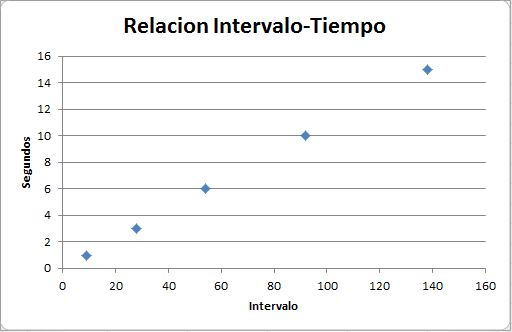
\includegraphics[width=0.80\textwidth, height = 7cm]{relacionintervalotiempo.JPG}
  \caption{Gráfico elaborado a partir de la tabla \ref{it5:tab:tablamediciones}, obtenido midiendo el tiempo entre cada medición para los intervalos en el eje de las abscisas. Observando la curva, llegamos a la conclusión que los distintos valores de tiempo correspondientes a los intervalos se comportan de manera lineal. Haciendo una extrapolación básica, podemos decir que el intervalo mas largo, con un valor de 65536, corresponde a un tiempo de aproximadamente 2 horas entre cada medición.}\label{it5:fig:relacionintervalotiempo}
\end{figure}

Las funciones "cambiar\_pin" y "analizar\_buffer" dentro del modulo de conversor, manejan los buffers y realizan las conversiones según las configuraciones. Ambas son ejecutadas cíclicamente en el modo de conversiones continuas. "cambiar\_pin" prepara el hardware del conversor según cual es el canal próximo a medir, y "analizar\_buffer" recorre el buffer, habilitando o no la conversión, y actualizándolo en cada corrida. Las figuras \ref{it5:fig:actividadanalizarbuffer} y \ref{it5:fig:actividadcambiarpin} describen las funciones con diagramas de actividad.
 
\begin{figure}[h]
  \centering
  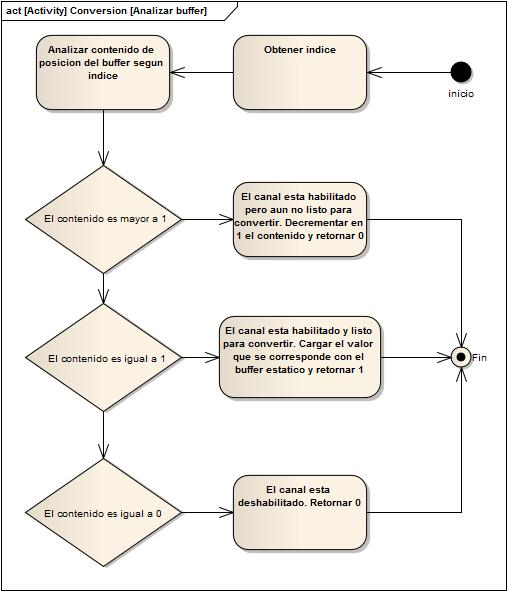
\includegraphics[width=1\textwidth, height = 12cm]{actividadanalizarbuffer}
  \caption[Diagrama de actividad de la función analizar buffer]{Diagrama de actividad que muestra el funcionamiento de la función analizar buffer. Esta función esta pensada para trabajar junto con "cambiar\_pin". En cada cambio de pin, se analiza el buffer para saber si hay que convertir o no, y actualizar el estado de los elementos del buffer, que corresponden en uno a uno con todas las vías de conversión posibles.}\label{it5:fig:actividadanalizarbuffer}
\end{figure}



\begin{figure}[h]
  \centering
  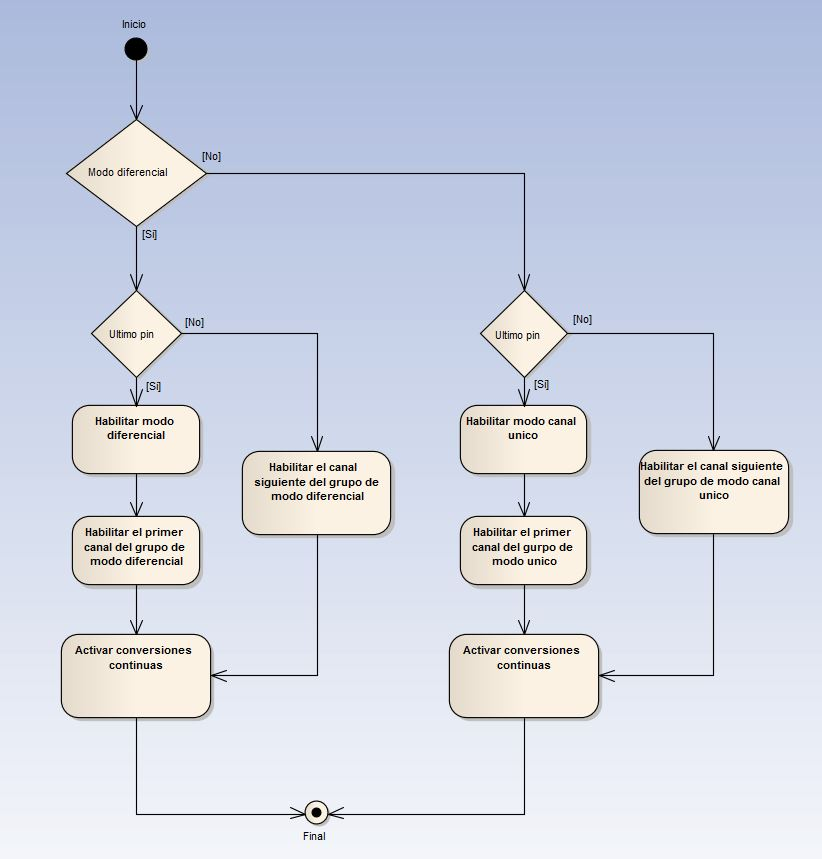
\includegraphics[width=1\textwidth, height = 12cm]{actividadcambiarpin}
  \caption[Diagrama de actividad de la función cambiar pin]{Diagrama de actividad que ilustra la lógica dentro de la función cambiar\_pin, dentro del modulo del conversor. Esta función es llamada luego de cada conversión. En cada llamado, se selecciona un nuevo canal a medir. No discrimina si el canal esta o no habilitado para medir, en caso en que no lo este, se llamara inmediatamente para cambiar el pin nuevamente sin realizar medición alguna.}\label{it5:fig:actividadcambiarpin}
\end{figure}

\subsubsection{Marca de tiempo} % (fold)
\label{ssub:marca_de_tiempo}

En algunos casos, puede ser necesario saber la hora, minuto y segundo en el que se midió. Para esto, sugerimos la idea de que se incluya una marca de tiempo dentro de los meta-datos enviados a la placa de gestión. Fue un requerimiento propuesto por nosotros en una etapa ya avanzada del proyecto. Esta marca de tiempo es necesariamente relativa al momento de inicio de conversiones continuas. Esto se debe a que la placa de instrumentación no tiene manera directa de calcular la fecha y hora exacta del día, por lo que obtener una marca de tiempo absoluta de manera directa en esta placa no es practico. 
La solución planteada para obtener una marca de tiempo absoluta fue calculándola en la placa de gestión. Al estar esta placa conectada a internet, puede obtener fácilmente la fecha y hora de inicio de conversiones. Con esto, a la fecha y hora se le suma la marca relativa de cada medición, y se obtiene así la marca de tiempo absoluta. Sabiendo esto, en esta sección explicamos la obtención de la marca de tiempo relativa. La marca de tiempo absoluta se obtiene usando la marca relativa junto con la fecha y hora actuales. Implica que deberá calcularse en un sistema con posibilidad de obtener esta información \\

El proceso para obtener la marca de tiempo esta descripto en la imagen \ref{it5:fig:secuenciaobtenermarca} mediante un diagrama de secuencia. La marca de tiempo relativa se obtiene con el uso del timer2. Esto significa reducir la cantidad de contadores de eventos disponibles de 2 a 1, lo cual afecta de manera directa a un requerimiento principal. La solución planteada fue dejar como opcional el calculo de la marca de tiempo, pudiendo así elegir el uso del timer2 entre contador de eventos o contador interno para la marca de tiempo. Esto es posible porque hay casos donde no es necesario ser preciso a la hora de tener el tiempo de las mediciones, y se pueden calcular las marcas directamente desde el sistema de gestión, y así dejar libre al Timer2 para el conteo de eventos. Esto fue un compromiso dado el estado avanzado del proyecto.


\begin{figure}[h]
  \centering
  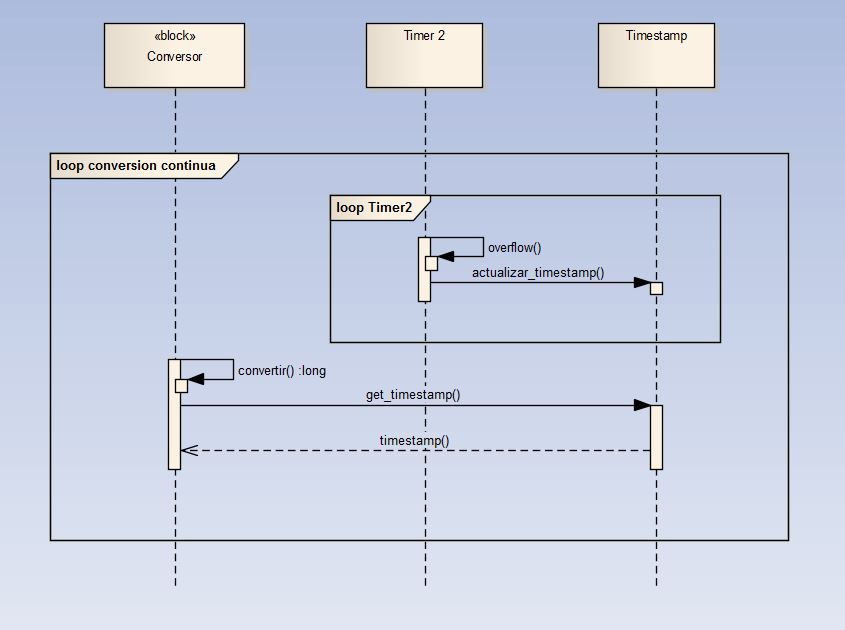
\includegraphics[width=1\textwidth, height = 9cm]{secuenciaobtenermarca}
  \caption[Diagrama de secuencia para la obtención de una marca de tiempo]{Diagrama de secuencia que muestra la interacción entre el conversor y Timer 2 para obtener la marca de tiempo. En el diagrama, la marca de tiempo esta representada mediante un objeto que alberga un único campo, que es la marca de tiempo. En cada interrupción de Timer 2 este valor se actualiza, y en cada conversión se obtiene el valor actual para enviarlo junto con la medición obtenida en la conversión.}\label{it5:fig:secuenciaobtenermarca}
\end{figure}

% subsubsection marca_de_tiempo (end)

% subsection conversor (end)

\subsection{Interfaz de usuario} % (fold)
\label{it5:sub:interfaz_de_usuario}

La interfaz de usuario siguió un diseño parecido al descrito en la sección \ref{it2:sub:logica_de_las_funciones_de_la_interfaz}. Gracias al diseño de la interfaz, agregar nuevos comandos con nuevos argumentos fue sencillo, siempre y cuando se respete la expresión regular.

Los comandos disponibles al final de esta iteración fueron:

\begin{itemize}
  \item SSE: - \textit{set single ended}: Establece un canal en modo único.
  \item SDI: - \textit{set differential}: Establece un par de canales en modo diferencial.
  \item GSE: - \textit{get single ended}: Obtiene una conversión instantánea en modo canal unico sobre un canal.
  \item GDI: - \textit{get differential}: Obtiene una conversión instantánea en modo diferencial sobre un par de canales.
  \item GDI: - \textit{get differential}: Obtiene una conversión instantánea en modo diferencial sobre un par de canales.
  \item SGA: - \textit{set gain}: Establece el nivel de ganancia del conversor.
  \item GT0: - \textit{get timer 0}: Obtiene el valor actual de la cuenta de timer 0, configurado como contador de eventos.
  \item GT2: - \textit{get timer 2}: Obtiene el valor actual de la cuenta de timer 2, configurado como contador de eventos.
  \item SHA: - \textit{show configuration}: Muestra la configuración actual de todos los canales y la ganancia del conversor.
  \item ST: - \textit{start}: Inicia el modo de conversiones continuas.
\end{itemize}

El conjunto entero de comandos esta documentado con mayor detalle en el apéndice \ref{ap:instrucciones}.
% subsection interfaz_de_usuario (end)

\subsection{Memoria flash} % (fold)
\label{it5:sub:memoria_flash}

La memoria flash del microcontrolador puede ser utilizada para guardar las configuraciones actuales, de forma que si el sistema se apaga, se pueda volver a iniciar con las configuraciones ya cargadas, sin necesidad de volver a establecer todo cada vez que se inicie nuevamente. Esto fue planteado como requerimiento para esta iteración, pero no pudo ser posible. Las operaciones necesarias para leer y escribir la memoria y el tamaño de la misma hicieron que sea difícil realizar la escritura y la lectura de la misma.

Tanto el programa que corre en el microprocesador como los datos de configuración debe guardarse en la misma memoria flash de 8Kb, siendo que el programa ocupa alrededor de 7Kb. En el Kb que resta, es posible guardar las configuraciones, pero el método de escritura de la flash pone en riesgo la integridad del programa. La única manera de escribir en memoria es haciéndolo sobre una pagina de 512 bytes. Dado el reducido espacio disponible, era probable que en una escritura se sobre escribiera parte del programa, haciendo que el sistema falle.
Teniendo en cuenta esto, se decidió no utilizar la flash para guardar las configuraciones. Por lo tanto, cada vez que el sistema se apague, se pierden las configuraciones, sin posibilidad de guardarlas.

% subsection memoria_flash (end)

% section desarrollo (end)

\section{Pruebas} % (fold)
\label{it5:sec:pruebas}

\begin{table}[h]
\centering
\caption{Test de sistema 1: Comportamiento esperado del conversor}
\label{it5:tab:testsistema1}
\begin{tabular}{p{2cm} p{9cm}}
\multicolumn{2}{c}{\cellcolor[HTML]{68CBD0}{\color[HTML]{000000} Prueba de sistema}} \\
Prueba \#        & 3 \\
\hline
Nombre           & Comportamiento esperado del conversor \\
\hline
Requerimiento & 1.5 \\
\hline
Descripción      & Con esta prueba, se comprueba que el sistema permite establecer intervalos de medición individuales para cada canal, y que se comporta de manera consistente con el el paso del tiempo. \\
\hline
Pre-condiciones  & \tabitem Sistema configurado con dos pines en modo canal único \\
                 & \tabitem Un canal esta configurado con un tiempo de 1 y otro con 50 \\
                 & \tabitem Generadores de tensión conectados a los pines configurados  \\
                 & \tabitem Computadora conectada al sistema mediante cable serial RS-232 \\
                 & \tabitem Lector de canal serial abierto en la computadora  \\
                 & \tabitem Sistema midiendo en modo de conversiones continuas\\
\hline

Post-condiciones & La frecuencia de medición para el canal en 1 debería ser mayor a la frecuencia del canal en 50.                     
\\
\hline
Secuencia  & \tabitem Establecimos una tensión de 1,5 voltios en el primer generador, conectado al canal con intervalo 1 y una de 2 voltios en el segundo, con intervalo 50 \\
\hline
Resultados       & El canal con intervalo 1 tenia una frecuencia mucho mayor al canal con intervalo 50, que era lo esperado. La relación entre las frecuencias parecía ser lineal (50 veces mas frecuente el primero que el segundo), aunque no teníamos una manera precisa de medirlo, mas que contar la cantidad de mediciones en un intervalo grande de tiempo.
\end{tabular}
\end{table}

\begin{table}[h]
\centering
\caption{Test de sistema 2: Generación de la marca de tiempo}
\label{it5:tab:testsistema2}
\begin{tabular}{p{2cm} p{9cm}}
\multicolumn{2}{c}{\cellcolor[HTML]{68CBD0}{\color[HTML]{000000} Prueba de sistema}} \\
Prueba \#        & 3 \\
\hline
Nombre           & Generación de la marca de tiempo \\                 
\hline
Requerimiento & 4.2 \\
\hline
Descripción      & En cada conversión, se debería registrar una marca de tiempo con un numero que hace referencia al tiempo que transcurrió desde el momento que se iniciaron las conversiones al momento donde se toma la medición. \\
\hline
Pre-condiciones  & \tabitem Sistema configurado con un pin en modo canal único, con un intervalo de 9, que corresponde a 1 segundo según la tabla \ref{it5:tab:tablamediciones} \\
                 & \tabitem Generador de tensión conectado al pin configurado  \\
                 & \tabitem Computadora conectada al sistema mediante cable serial RS-232 \\
                 & \tabitem Lector de canal serial abierto en la computadora  \\
                 & \tabitem Cronometro en 00:00\\
                 & \tabitem Reloj en hora\\
\hline

Post-condiciones & La diferencia entre cada marca de tiempo y la siguiente debería ser constante, y debería ser aproximada al valor en segundos dado por el intervalo. El calculo en fecha y hora de la ultima marca de tiempo y el valor del cronometro (hecho con ayuda del reloj) debería dar aproximadamente igual. \\
\hline
Secuencia  & \tabitem Establecimos una tensión en el generador. \\
           & \tabitem Iniciamos las conversiones continuas. \\
           & \tabitem Dimos arranque al cronometro. \\
           & \tabitem Medimos el tiempo entre cada medición con ayuda del cronometro en 30 mediciones sucesivas. \\

Resultados       & Los resultados fueron los esperados. El intervalo de tiempo entre cada medición era aproximadamente 1 segundo en todos los casos. Lo que significa que el tiempo entre cada medición no varia con el paso del tiempo para un intervalo constante. 
\end{tabular}
\end{table}

\begin{table}[h]
\centering
\caption{Test de sistema 3: Formato esperado del mensaje}
\label{it5:tab:testsistema3}
\begin{tabular}{p{2cm} p{9cm}}
\multicolumn{2}{c}{\cellcolor[HTML]{68CBD0}{\color[HTML]{000000} Prueba de sistema}} \\
Prueba \#        & 3 \\
\hline
Nombre           & Formato esperado del mensaje \\                     
\hline
Requerimiento    & 4.3, 4.4, 4.5 \\
\hline
Descripción      & Cada dato que se envía a la placa de gestión incluye la siguiente información: Medición, pin, modo, marca de tiempo. Estos datos están enviados con un formato especial, y se envían en simultaneo. Esta prueba verifica que cada mensaje contenga el formato correcto y que los datos sean coherentes a las configuraciones. \\
\hline
Pre-condiciones  & \tabitem Sistema configurado con el pin 3 en modo canal único, con un intervalo de 10 \\
                 & \tabitem Generador de tensión conectado al pin configurado con un valor de 1,5 volts  \\
                 & \tabitem Computadora conectada al sistema mediante cable serial RS-232 \\
                 & \tabitem Lector de canal serial abierto en la computadora  \\
                 & \tabitem Sistema midiendo en modo de conversiones continuas\\
\hline

Post-condiciones & El mensaje recibido en el lector serial debería ser "1500,3,SE,[marca de tiempo]".                     
\\
\hline
Resultados       & El formato era correcto
\end{tabular}
\end{table}

% section pruebas (end)

\section{Conclusiones} % (fold)
\label{it4:sec:conclusiones}

Algunos de los requerimientos principales y secundarios no se llegaron a cumplir por inconvenientes en el desarrollo, pero se tomaron ciertas medidas para compensar los problemas, sobretodo en aquellos que involucraban a los requerimientos principales y de mayor riesgo:

\begin{itemize}
\item Guardar las configuraciones y parámetros del programa en la memoria flash no fue posible debido al poco espacio dentro de la memoria, y la impracticidad del método de escritura y lectura. Este no era un requerimiento principal, por lo que decidimos descartarlo.
\item La cantidad de contadores de eventos paso de 4 a 2 debido a la naturaleza de los mismos y el uso del modulo UART del microcontrolador. Tener 4 contadores de eventos es condicion necesaria, ya que es uno de los requerimientos principales [1.3]. La solucion a este problema se planteara en la proxima iteración.
\end{itemize}

A pesar de no estar completo aún, el software de la plataforma es estable y funcional. Los tests unitarios aseguran la respuesta necesaria ante cualquier error por parte del usuario. Además, el hecho que no sea un software de gran tamaño permite que no se congele en medio de una ejecución, interrumpiendo una sesión de adquisición de datos. A continuación listamos las funcionalidades principales desarrolladas, en esta iteración, según los requerimientos principales.

\begin{itemize}
\item Es posible configurar tiempos de intervalo entre cada medición para cada canal por separado (cumple con 1.5)
\item Los datos que se envían a la placa de gestión para cada medición incluyen, además de la medición, el numero de pin o pines (si es modo diferencial) de donde se esta midiendo. (cumple con 4.3)  
\item Los datos que se envían a la placa de gestión para cada medición incluyen, además de la medición, el modo de conversión del canal por donde se esta midiendo. (cumple con 4.4)
\item Los datos que se envían a la placa de gestión para cada medición incluyen, además de la medición, la marca de tiempo relativa correspondiente de la medición hecha. (cumple con 4.5)
\end{itemize}

El requerimiento 4.1 no pudo ser cumplido debido a complicaciones con el modulo flash del microcontrolador, y se probara el cumplimiento del requerimiento 4.2 cuando se cuente con un sistema embebido que pueda generar marcas de tiempo absolutas.

% section conclusiones (end)

% chapter iteracion_4 (end)